\chapter{Scaling Analysis and Benchmarking}
\label{chap:scaling}

Having established the analytical gradient expressions and their numerical evaluation in Chapter~\ref{chap:grape}, this chapter presents a systematic comparison of three methods for computing gradients within GRAPE: evaluation of hard-coded gradients (HG), full automatic differentiation (full-AD)~\cite{pacleung2017speedup}, and semi-automatic differentiation (semi-AD)~\cite{semiadgoerz2022quantum}. To determine the method most appropriate for a given problem, I inspect the memory usage and runtime scaling of these three approaches. Following this analysis, I present benchmark studies of specific state-transfer and gate-operation problems to illustrate the scaling behavior.

\section{Scaling analysis of runtime and memory usage}
\label{sec:scaling_analysis}

Runtime and memory usage can pose significant challenges when performing optimization tasks for quantum systems with large Hilbert space dimension ($d$) or for time evolution requiring a significant number of time steps ($N$). In this section, I analyze the scaling of memory usage and runtime with respect to both $N$ and $d$, focusing on the cost contribution $C_1$ for state-transfer and unitary-gate optimization. The findings can be generalized to other cost contributions beyond $C_1$.

\subsection{Hard-coded gradients via forward-backward propagation}
\label{sec:HG_scaling}

I start by considering state-transfer problems. The \textit{memory usage} for evaluating $\nabla C_1^{st}$ is mainly determined by the required storage of quantum states and the Hamiltonian. In forward-backward propagation, the number of states and instances of Hamiltonian matrices stored at any given time is of the order of unity. Each individual state vector of dimension $d$ consumes memory $\sim\Theta(d)$. Memory usage for the Hamiltonian depends on the employed storage scheme. In the ``worst'' case of dense matrix storage, the memory required for the Hamiltonian is $\Theta(d^2)$. For sparse matrix storage, memory usage generally depends on sparsity and is determined by the number of stored Hamiltonian matrix elements (here denoted as $\kappa$).%
\nomenclature{$\kappa$}{Number of stored Hamiltonian matrix elements}
For example, for a diagonal or tridiagonal matrix, memory usage is $\kappa\sim\Theta(d)$; for a linear chain of qubits with nearest-neighbor $\sigma_z$ coupling, it is $\Theta(d\, \log_2 d)$. Combining the scaling relations above gives an overall asymptotic behavior of memory usage $\Theta(d+\kappa)$.

The \textit{runtime} of the scheme is dominated by the required $\Theta(N)$ evaluations of propagator-state products and their derivative counterparts. Numerically approximating a single propagator-state product requires $\mu$ matrix-vector multiplications [see Eq.~\eqref{eq:mudefnition}], where the runtime of one instance of matrix-vector multiplication scales as $\Theta(\kappa)$.  The implicit dependence of $\mu=\mu(d)$ on $d$ is specific to each particular system and can be difficult to obtain analytically. Numerically, I find for a driven transmon coupled to a cavity that $\mu\sim\Theta(\sqrt{d})$; for a linear chain of coupled qubits, the scaling is $\Theta(\log_2 d)$; see Appendix~\ref{app:muscaling} for more details. 
Once combined, the above individual scaling relations lead to an overall runtime asymptotic behavior 
$\Theta(N\mu\, \kappa)$. For example, in the case of the linear chain of coupled qubits, runtime scales as $\Theta(Nd\, (\log_2 d )^2)$.

For gate-optimization problems, the scaling behavior of memory usage and runtime is as follows. The gradient $\nabla C_1^{ g}$ is calculated by sequentially 
applying forward-backward propagation to each of the $d$ basis states. The memory usage is $\Theta(d+\kappa)$, the same as for $\nabla C_1^{st}$. The runtime scaling is $\Theta(N\mu\kappa d)$, which is $d$ times larger than the runtime scaling for $\nabla C_1^{st}$. (Another way of calculating $\nabla C_1^{ g}$ consists of parallelized forward-backward propagation of all basis states. The concrete scaling behavior then depends on the parallelization scheme; that discussion is beyond the scope of this thesis.)

Thanks to the similarities in the expressions and the existence of recursion relations, forward-backward schemes akin to Fig.~\ref{fig:GRAPE} 
can also be applied to $\nabla C_2^{st}$, $\nabla C_3^{st}$, and $\nabla C_3^{g}$. As a result, the scaling analysis leads to the same memory usage and runtime requirements as $\nabla C_1^{st}$ and $\nabla C_1^{g}$.



\subsection{Full automatic differentiation}
\label{sec:fullAD_scaling}

Reverse-mode automatic differentiation extracts gradients by a forward pass and a reverse pass through the computational tree. With the forward pass the cost function $C$ is computed, and the backward pass accumulates the gradient via the chain rule.

The \textit{memory usage} for evaluating $\nabla C_1^{st}$ is determined by the requirement that all intermediate numerical results must be stored as part of the forward pass and act as input to the reverse pass. Specifically, as shown in Fig.~\ref{fig:GRAPE}, the forward pass evolves the initial state vector to the final state vector in $N$ time steps. The total number of vectors that have to be stored along the way is $\Theta
(N\mu)$, since computation of a single short-time propagator-state product via scaling and squaring necessitates $\mu$ iterations. In addition, considering the memory usage for the Hamiltonian, the full scaling is $\Theta(N\mu d +\kappa)$. 

The \textit{runtime} for evaluating $\nabla C_1^{st}$ combines forward and reverse passes. It is dominated by the evaluation of $\Theta(N)$ propagator-state products, each of which has the runtime scaling $\Theta(\mu\kappa)$, leading to an overall runtime scaling of $\Theta(N\mu \kappa )$.

For gate-optimization problems, $C_1^{ g}$ is evaluated by evolving not only a single initial state but a whole set of $d$ basis vectors. Evaluating $Nd$ propagator-state products requires $\Theta(N\mu d^2+\kappa)$ memory, where the number of stored Hamiltonian matrix elements $\kappa$ takes into account storage of the Hamiltonian. Since $\kappa$ has the worst-case scaling $\Theta(d^2)$ in the case of a dense Hamiltonian matrix, the overall scaling is $\Theta(N\mu d^2)$. Assuming that the evolution of individual basis vectors is not parallelized, runtime also grows by a factor of $d$, so that runtime scaling for $\nabla C_1^{ g}$ is $\Theta(N\mu\kappa d)$.

Despite the specific differences among the expressions of cost contributions $C_2^{st}$, $C_3^{st}$, and $C_3^{g}$, the scaling of runtime and memory usage is again set by the need to store intermediate vectors and repeatedly perform matrix-vector multiplications. Consequently, the scaling remains the same as for the cost contributions discussed above.

\subsection{Semi-automatic differentiation}
\label{sec:semiAD_scaling}

For gradients of cost contributions that are tedious to derive analytically, semi-automatic differentiation~\cite{semiadgoerz2022quantum} offers an alternative approach in which some derivatives are hard-coded and others treated by automatic differentiation. Compared to full-AD, semi-AD has the benefit that the memory usage scaling is independent of $\mu$ while maintaining the same runtime scaling. 

\subsection{Comparison}
\label{sec:scaling_comparison}

\begin{table}[t]
\renewcommand{\arraystretch}{1.5}
\centering
\caption[Memory usage and runtime scaling with respect to Hilbert space dimension $d$, number of time steps $N$, the number of stored Hamiltonian matrix elements $\kappa=\kappa(d)$, and the number of matrix-vector multiplications required for evaluating propagator-state products $\mu=\mu(d)$.]{Memory usage and runtime scaling with respect to Hilbert space dimension $d$, number of time steps $N$, the number of stored Hamiltonian matrix elements $\kappa=\kappa(d)$, and the number of matrix-vector multiplications required for evaluating propagator-state products $\mu=\mu(d)$. (The scaling of $\mu$ and $\kappa$ depends on the specific optimization task.) The table contrasts scaling for state transfer and gate operation for hard-coded gradients (HG), full automatic differentiation (full-AD), and semi-automatic differentiation (semi-AD).}
\label{tab:scalingtable}
\begin{tabular}
{p{0.27\textwidth}p{0.13\textwidth}p{0.17\textwidth}p{0.13\textwidth}p{0.17\textwidth}} 
\hline
\hline
& \multicolumn{2}{c}{\textbf{\textsc{State transfer}}} & \multicolumn{2}{c}{\textbf{\textsc{Gate operation}}}\\
\hline 
& \textbf{Runtime} & \textbf{Memory usage} & \textbf{Runtime} & \textbf{Memory usage}
\\
\hline
HG & $\Theta(N\mu \kappa)$ & $\Theta(d+\kappa)$ & $\Theta(N\mu \kappa d)$ & $\Theta(d+\kappa)$\\ 
Full-AD & $\Theta(N\mu \kappa)$ & $\Theta(N\mu d+\kappa)$ & $\Theta(N\mu \kappa d)$ & $\Theta(N\mu d^2)$  \\
Semi-AD & $\Theta(N\mu \kappa)$ & $\Theta(Nd+\kappa)$ & $\Theta(N\mu \kappa d)$ & $\Theta(Nd^2)$\\ 
\hline \hline
\end{tabular} 
\end{table}

The results of this scaling analysis are summarized in Table~\ref{tab:scalingtable}. For full-AD, memory usage grows linearly with respect to $\mu$ and number of time steps $N$. By contrast, memory usage for HG does not increase with $\mu$ and $N$, but remains constant. This advantage is not bought at the cost of worse runtime scaling. Therefore, HG is preferable over full-AD in the optimal control of large quantum systems where memory usage would otherwise be prohibitively large. Semi-AD presents an interesting compromise viable whenever the memory bottleneck is not too severe. Note that the runtime scaling $\Theta(N\mu\kappa d)$ of HG via scaling and squaring can in principle exceed the scaling $O(Nd^3)$ for matrix exponentiation based on matrix diagonalization (see Appendix~\ref{app:matdiag}). In that case, the latter is the better option.

I illustrate the discussed scaling by benchmark studies for concrete optimization problems in the following section.


\section{Benchmark studies}
\label{sec:benchmarks}

\subsection{State-transfer benchmark}

The first benchmark example studies the following state-transfer problem. Consider a setup in which a driven flux-tunable transmon is capacitively coupled to a superconducting cavity, and perform a state transfer from the cavity vacuum state to the 20-photon Fock state. The Hamiltonian in the frame co-rotating with the transmon drive is
\begin{equation}
\label{eq:fockH}
    H_1(t)=\Delta b^\dagger b+\frac{1}{2}\alpha b^\dagger b(b^\dagger b-1)+g(cb^\dagger+c^\dagger b)+a_{z}(t)b^\dagger b
    +a_{x}(t)(b+b^\dagger).
\end{equation}
Here, the drive is both longitudinal and transverse; $c$ and $b$ are the annihilation operators for cavity photons and transmon excitations, respectively. $\alpha$, $g$, and $\Delta$ denote anharmonicity, interaction strength, and the difference between the transmon and cavity frequencies. 
 
Optimization proceeds by minimizing the infidelity $C_1^{st}$ and limiting the occupation of higher transmon levels by including the cost contribution $C_2^{st}$ [Eq.~\eqref{eq:c2st}]. The latter has the additional benefit of enabling the truncation to only a few transmon levels. I measure runtime and peak memory usage of full-AD,\footnote{AD is implemented by the package \texttt{Autograd}~\cite{maclaurin2015autograd} in this benchmark. This package does not support sparse linear algebra, so I implement dense matrix storage for the Hamiltonian in both full-AD and HG for fair comparison.} semi-AD, and HG for a single optimization iteration. The runtime is measured by the package \texttt{Temci}~\cite{temci} and
the peak memory usage is monitored by the \texttt{memory\_profiler} package~\cite{memory}. The optimization is performed on an AMD Ryzen Threadripper 3970X 32-Core CPU with 3.7\,GHz frequency. 


\begin{figure}[t]
  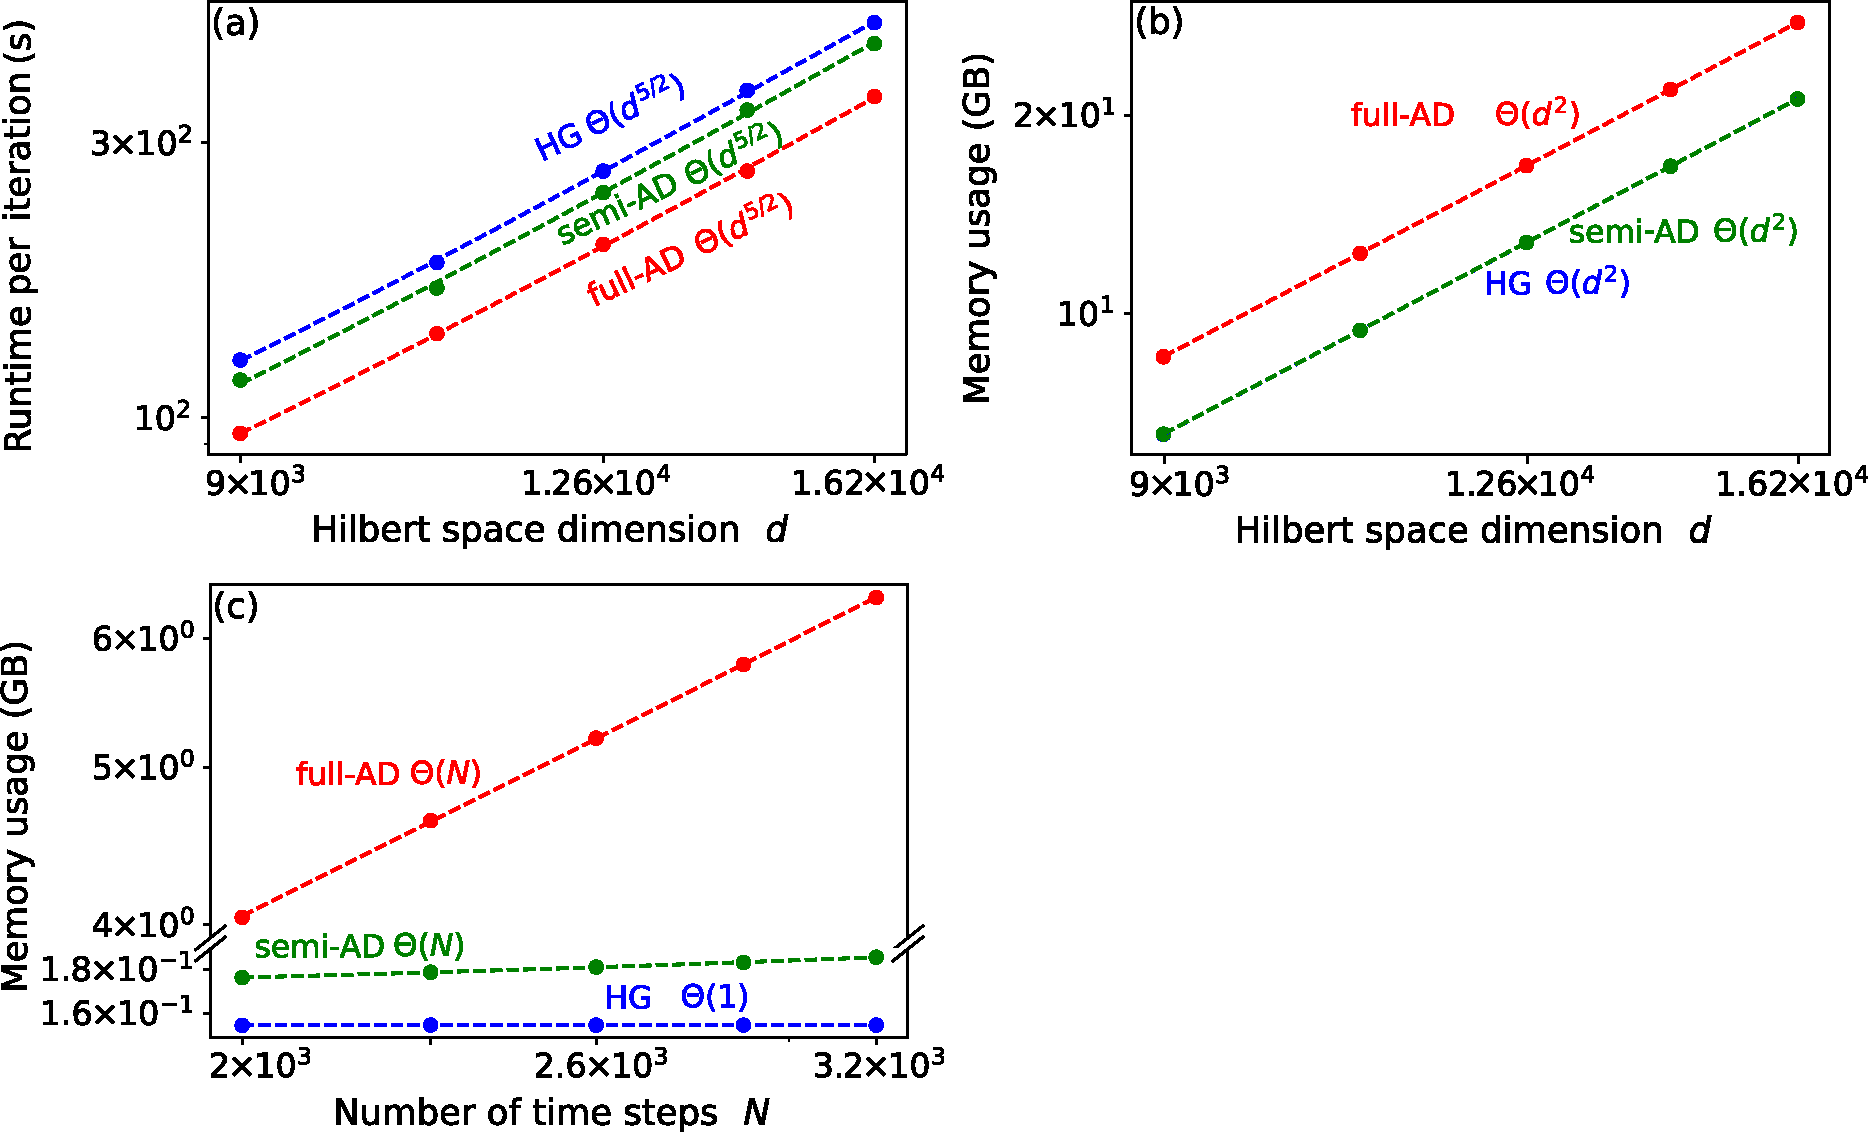
\includegraphics[width=\linewidth]{ch3_figures/state.pdf} 
  \caption[Benchmark results for Fock state generation in a system consisting of a cavity coupled to a transmon.]{Benchmark results for Fock state generation in a system consisting of a cavity coupled to a transmon. (a)~Runtime per iteration and (b)~memory usage versus Hilbert space dimension $d$. The dimension is varied by increasing the cavity dimension while fixing the transmon dimension to 6. (c)~Memory usage as a function of the number of time steps for $d=240$. All plots are in log-log scale. Dashed lines are power-law fits. (Parameters: $\Delta/2\pi=3\,$GHz, $g/2\pi=0.1\,$GHz, $\alpha/2\pi=-0.225\,$GHz, and constant controls $a_z/2\pi=a_x/2\pi=0.1\,$GHz.)}
  \label{fig:state_time}
\end{figure}

Benchmark results for the state-transfer optimization are shown in Fig.~\ref{fig:state_time}. I consider a single time step ($N=1$) and measure the runtime versus $d$. The results in Fig.~\ref{fig:state_time}(a) confirm that full-AD, semi-AD, and HG have the same scaling of runtime per time step with respect to $d$ (Table~\ref{tab:scalingtable}). The observed runtime scaling $\Theta(d^{5/2})$ is consistent with $\kappa \sim \Theta(d^2)$ due to dense matrix storage for $H_1$, and $\mu\sim \Theta(d^{1/2})$ (see Appendix~\ref{app:muscaling}). The scaling of the required memory resources is illustrated in Fig.~\ref{fig:state_time}(b): memory usage scales with dimension $d$ as $\Theta(d^2)$ for full-AD, semi-AD, and HG, consistent with $\kappa\sim \Theta(d^2)$ being the dominant contribution. As anticipated, the scaling of memory with $N$ differs between full-AD, semi-AD, and HG [Fig.~\ref{fig:state_time}(c)]. For full-AD and semi-AD, the scaling is linear with $N$, while it is independent of $N$ for HG. The slope of full-AD is much larger than the one of semi-AD, since the former has extra dependence on $\mu$ (Table~\ref{tab:scalingtable}), which is a constant $\approx 100$ in this benchmark. The results confirm the favorable memory efficiency of HG and semi-AD compared to full-AD in state-transfer problems with large number of time steps. 

\subsection{Gate-operation benchmark}

I next turn to an example for optimizing a unitary gate. This benchmark is performed for three driven transmons with nearest-neighbor coupling. The target gate consists of simultaneous Hadamard operations on each of the three transmons. For concreteness, I consider the case of transmons with the same frequency, driven resonantly. The full Hamiltonian in the rotating frame of the drive is
\begin{equation}
\label{eq:gateH}
    H_2(t)=\sum_{\nu=1}^{3}\bigg[\frac{1}{2}\alpha b_\nu^\dagger b_\nu (b_\nu^\dagger b_\nu-1)+a^{(\nu)}(t)(b_\nu+b_\nu^\dagger)\bigg]+g(b_1b_{2}^\dagger+b_2b_{3}^\dagger+\text{h.c.}).
\end{equation}
The goal of the optimization is to minimize the infidelity $C_2^{ g}$. The setup for this benchmark is the same as in the previous example.

\begin{figure}[t]
  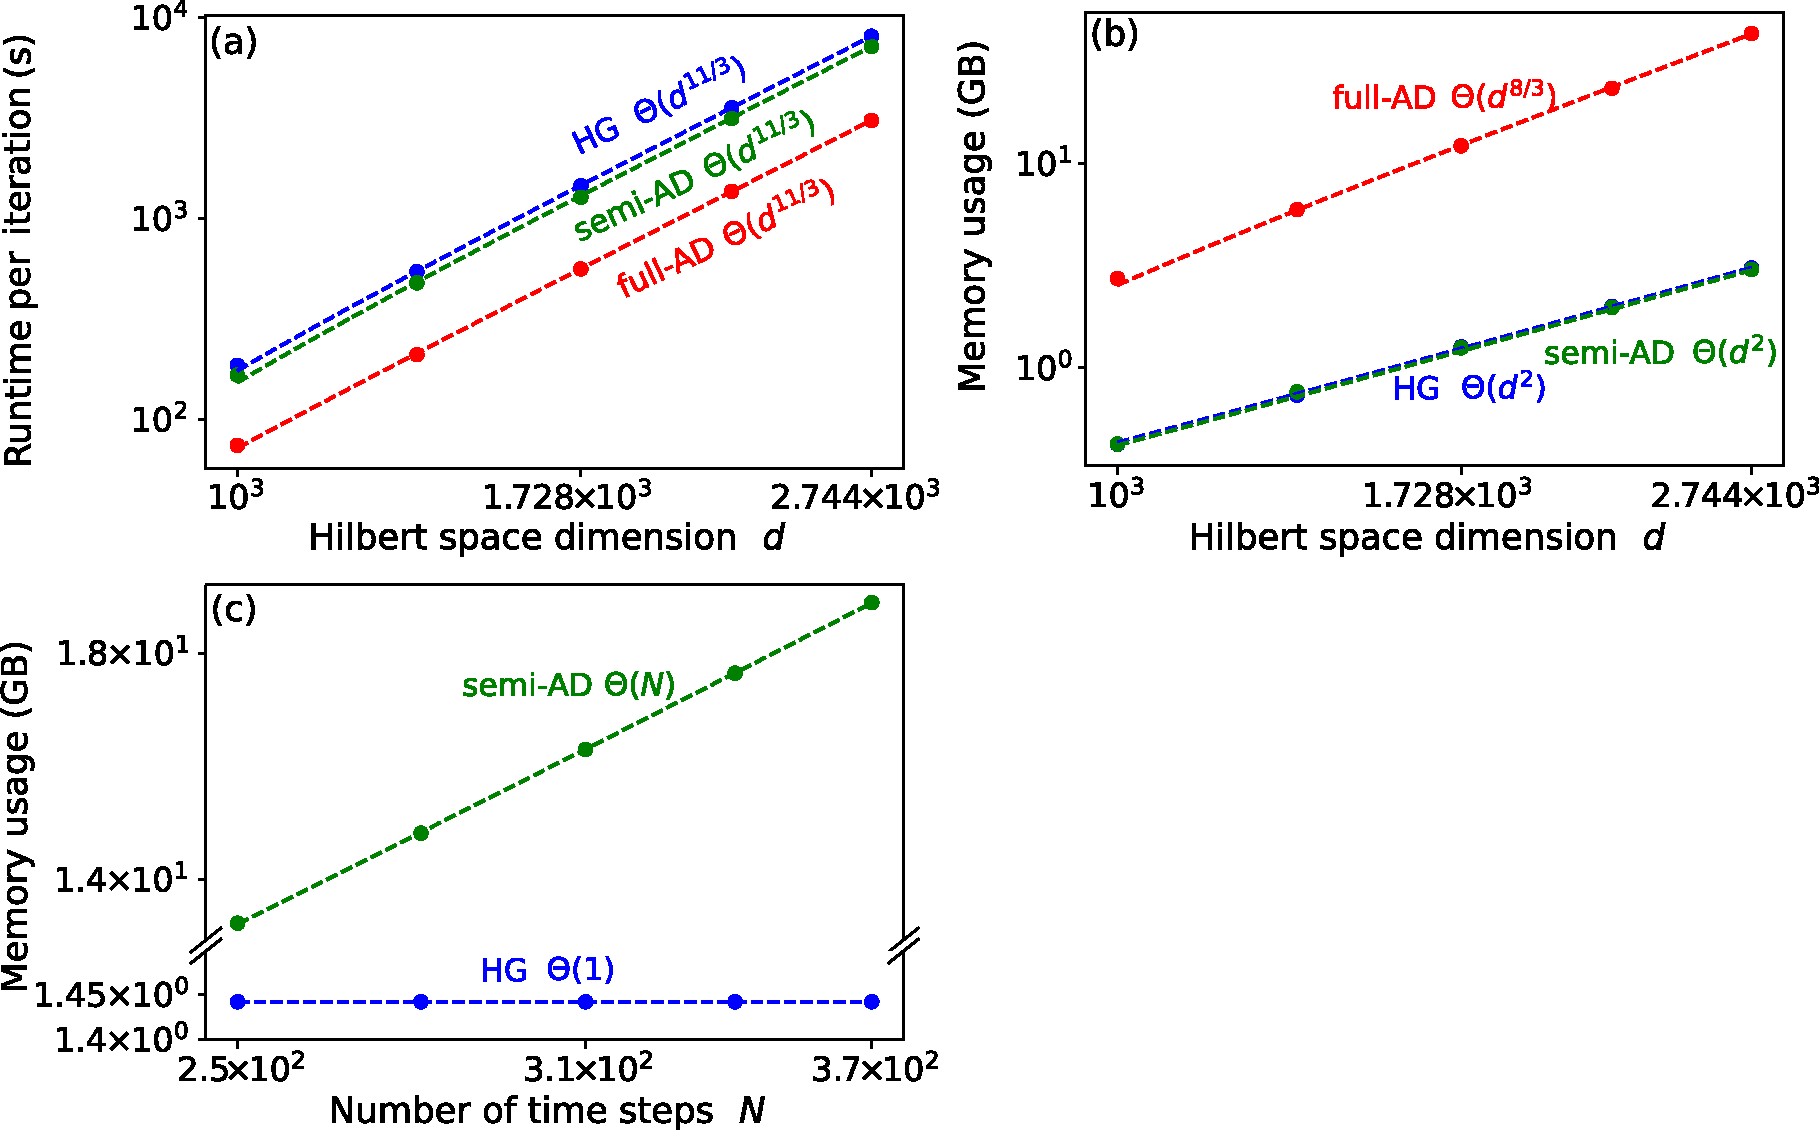
\includegraphics[width=\linewidth]{ch3_figures/gate.pdf}
  \caption[Benchmark results for unitary gate optimization in a system consisting of three coupled transmons.]{Benchmark results for unitary gate optimization in a system consisting of three coupled transmons. (a)~Runtime per iteration and (b)~memory usage versus Hilbert space dimension $d$. The total Hilbert space dimension $d$ is increased by enlarging the cutoff of each transmon from 10 to 14 simultaneously. (c)~Memory usage as a function of the number of time steps for $d=12^3=1728$. Full-AD (not shown) would require more memory than available resources (estimated: 1\,TB). All plots are in log-log scale. Dashed lines are power-law fits. (Parameters: $g/2\pi=0.1\,$GHz, $\alpha/2\pi=-0.225\,$GHz, and $a^{(\nu)}/2\pi=0.1\,$GHz.)}
  \label{fig:gate}
\end{figure}



Fig.~\ref{fig:gate} records the benchmarks based on a single time step ($N=1$). The observed runtime scaling with dimension $d$ is $\Theta(d^{11/3})$ for full-AD, semi-AD, and HG, see Fig.~\ref{fig:gate}(a). This power law arises from $\Theta(\mu\kappa d)$ for $\kappa\sim \Theta(d^2)$ and $\mu\sim \Theta(d^{2/3})$ [see Appendix~\ref{app:muscaling}]. The memory usage scaling with $d$ is illustrated in Fig.~\ref{fig:gate}(b), confirming that full-AD has an unfavorable extra $\mu \sim \Theta(d^{2/3})$ dependence compared to HG and semi-AD (Table~\ref{tab:scalingtable}). The memory usage scaling with $N$ is as expected [Fig.~\ref{fig:gate}(c)]: for semi-AD, the scaling is linear with $N$; for HG, it is independent of $N$. (The memory usage of full-AD in this case exceeds available resources, and thus is not shown.) Throughout this benchmark, this linear dependence with $N$ causes semi-AD to consume about 10 times more memory than HG. This underlines that HG is preferable whenever memory constraints become a limitation in optimization problems with large Hilbert space dimension and large number of time steps. This improvement is achieved without worsening the runtime scaling. 


\section{Choosing among different optimization strategies}
\label{sec:decision_tree}

\begin{figure}[t]
\centering
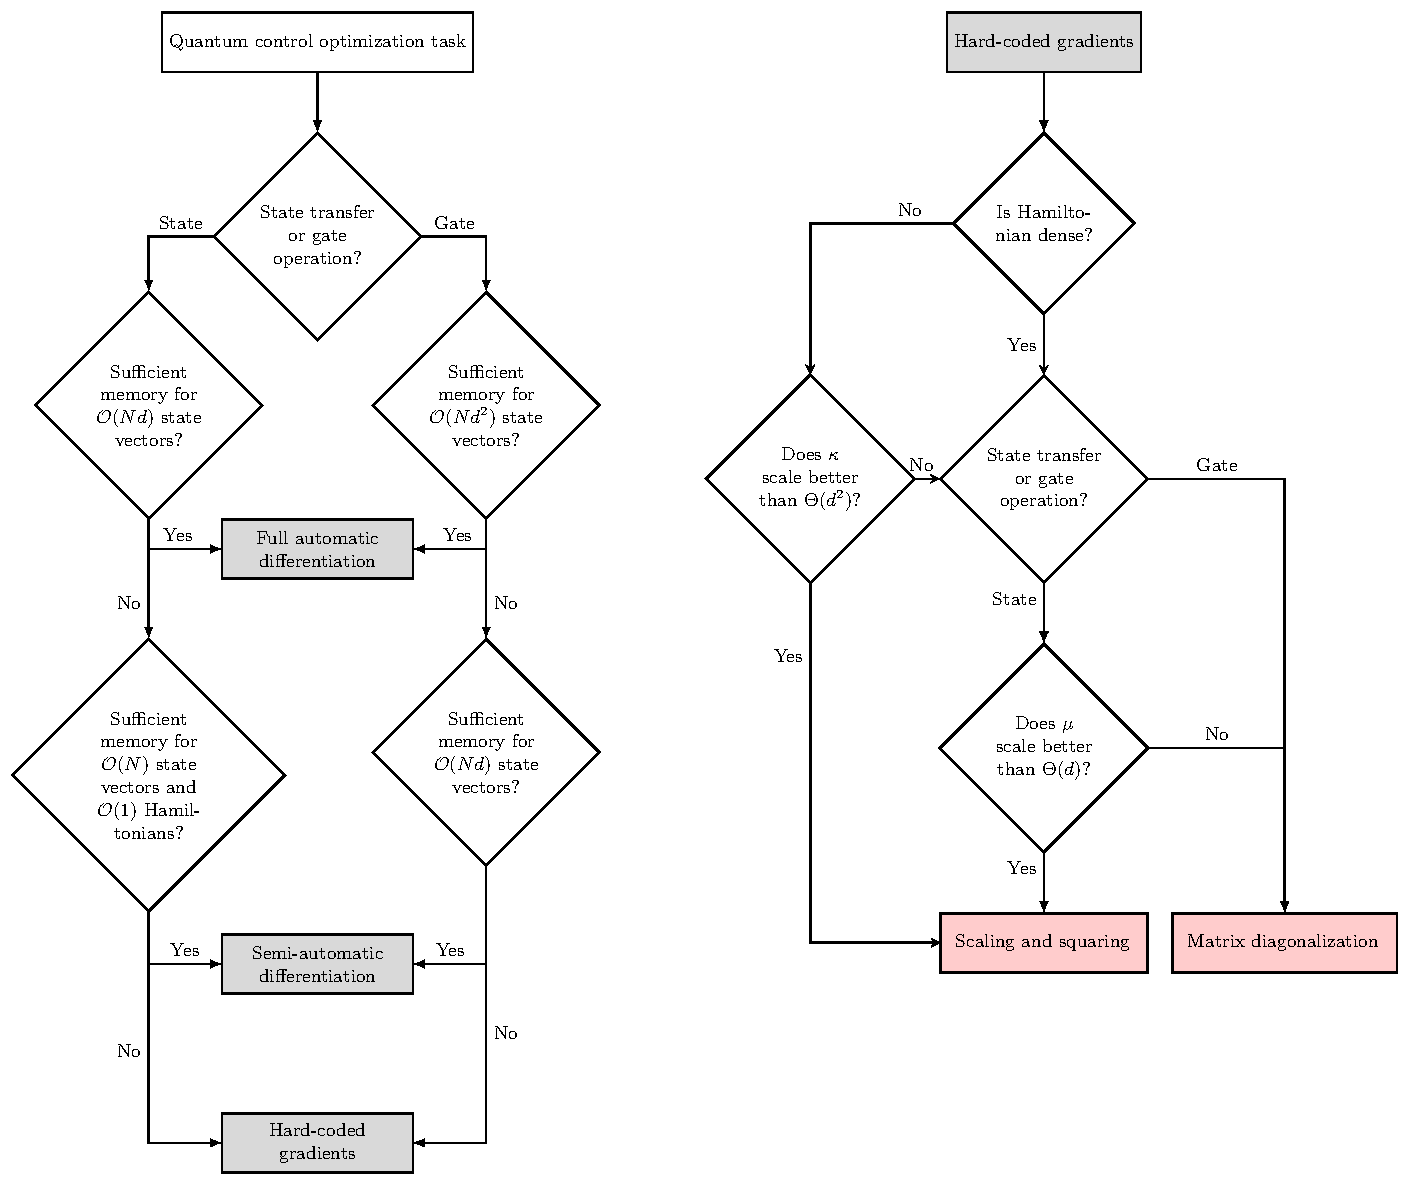
\includegraphics[width=\linewidth]{ch3_figures/decision_tree.pdf}
\caption[Decision trees for selecting the optimal numerical strategy.]{Decision trees for selecting the optimal numerical strategy. (a)~Choosing among three numerical methods for evaluating gradients: full automatic differentiation, semi-automatic differentiation, hard-coded analytical gradients. (Here, $\mu\sim\Theta(d)$ is assumed; for different scaling see Table~\ref{tab:scalingtable}.) (b)~Determining the appropriate strategy for evaluating propagator-state products.}
\label{fig:decision_tree}
\end{figure}

There are several considerations which determine whether full-AD, HG, or semi-AD is the optimal strategy for a given optimization problem, see the decision tree in Fig.~\ref{fig:decision_tree}. Whenever the Hilbert space dimension $d$ and the number of time steps $N$ are sufficiently small, memory usage may not be a bottleneck. In this case, full-AD may be preferable, since it eliminates the need for hard-coded gradients. If the memory cost of full-AD is not affordable but analytical gradients are tedious to compute, semi-AD may be a viable compromise, though still less memory efficient than HG. In all other cases, HG is the method of choice, since it can handle optimization with larger $N$ and $d$ compared to full-AD and semi-AD. 

The choice of implementing HG via scaling and squaring or matrix diagonalization should be informed by whether the Hamiltonian is sparse and $\kappa$ scales better than $\Theta(d^2)$. In the latter case, scaling and squaring is preferable and leads to an overall memory usage $\sim \Theta(d+\kappa)$, which is better than the memory scaling $O(d^2)$ of matrix diagonalization. By contrast, for Hamiltonians with $\kappa\sim \Theta(d^2)$, these two methods are equivalent in memory usage scaling, and the one with better runtime for a specific optimization task should be selected. While the runtime for optimization using matrix diagonalization scales as $O(d^3)$ [Appendix~\ref{app:matdiag}], the runtime for optimization based on scaling and squaring differs between state-transfer and gate optimizations: (1)~for state transfer, the runtime scales as $\Theta(\mu d^2)$; hence, whenever $\mu$ scales better than $\Theta(d)$, scaling and squaring wins over matrix diagonalization; (2)~for gate optimization, the runtime scales as $\Theta(\mu d^3)$; hence matrix diagonalization is preferable. 

The scaling analysis and benchmarks presented in this chapter confirm that hard-coded gradients provide the most memory-efficient approach for GRAPE-based optimization of large quantum systems. In the next chapter, I apply these insights to a concrete problem: designing detuning-robust control pulses for transmon gates.
